\newpage


\begin{subbox}{subbox}{}
\centering
\Large{\textbf{Network Science   \\ Cheatsheet}}
\end{subbox}

\begin{multibox}{2}
\begin{subbox}{subbox}{}
\centering

\includegraphics[width=0.8\textwidth]{pics/logo.png}
\end{subbox}
\begin{subbox}{subbox}{}
\centering
Made by \\
\large{
Remy Cazabet
}
\end{subbox}
\end{multibox}
\section{Blocks and Community structure}

\begin{textbox}{Blocks and Communities: Definition}
The general idea of blocks and communities is that nodes of a network can be grouped together in homogeneous sets, based on the network topology. The problem of automatically discovering those groups is one of the most studied problem of network science, but also one of the most poorly defined.

\end{textbox}

\begin{textbox}{Block structure}
The general idea of the block structure is that the probability to observe an edge between two nodes is a function of the blocks they belong to. Usually, no assumption is made apriori about those probabilities: they can be high between nodes belonging to the same blocks or to different blocks, and can differ for each pair of block.

This definition thus defines a random graph model, related to the ER random model, known as the \textbf{Stochastic block model}. 
\end{textbox}

\begin{textbox}{Community structure}
The idea of having a network structured in \textbf{communities} is defined as an analogy with communities in social networks. Communities are therefore defined (informally) as groups of nodes that are strongly connected between themselves (\textbf{high internal density}) and more weakly connected to the rest of the network \textbf{low external density}.

This definition however cannot be translated unambiguously into a mathematical formulation. The problem of \textbf{community detection}, or community discovery, is therefore complicated to define.
\end{textbox}

\begin{textbox}{Partitions/Overlap}
We must differentiate two types of node grouping: 
\begin{enumerate}
    \item A \textbf{Partition} of a graph is a division of its nodes such as each of them belong to one and only one group.
    \item Overlapping communities/blocks allow, on the contrary, nodes belonging to several groups. Unless specified differently, they also allow nodes to belong to no group.
\end{enumerate}
Algorithms searching partitions are much more common than those searching for overlapping groups, due to the increased complexity of the later task. Overlapping community detection is, nevertheless, an active field of research.
\end{textbox}

\begin{textbox}{Definition}
\begin{tabular}{p{0.08\textwidth}|p{0.8\textwidth}}\scriptsize

$C$ & a \textit{community partition}, or, more generally, a set of set of nodes \\
$c_i$ & community $i$, a set of nodes \\
\end{tabular}
\end{textbox}


\begin{textbox}{Modularity}
The most famous quality function to measure the \textit{quality} of partitions is called the \textbf{Modularity}. Introduced in \footcite{girvan2002community}, it is defined for a partition $C$ and a graph $G$ as the difference between the fraction of observed internal edges and the expected fraction of internal edges if $G$ were rewired according to a configuration model, i.e., preserving the degrees of nodes.

More formally, 
\[
Q=\frac{1}{L}\sum_{i=1}^{|C|}(L_{i}-\frac{1}{2}K_i^2)
\]
with $L_{i}=L(H(c_i))$ the number of edges inside community $i$ and $K_i=\sum_{u \in c_i}k_u$ the sum of degrees of nodes in community $i$.

The original formulation of modularity, often found in the literature, is:
\[
Q=\frac{1}{2L}\sum_{uv}\left[ A_{uv}-\frac{k_uk_v}{2L}\right] \delta(c_u,c_v)
\]
with $\delta(c_u,c_v)$ the kronecker delta between communities, i.e., $\delta(c_u,c_v)=1$ if nodes $u$ and $v$ belongs to the same community, 0 otherwise.


\end{textbox}

\begin{textbox}{Modularity: null model}
The modularity as expressed above compares the number of edges inside communities to the expected number of edges in a \textbf{null model}, i.e., a randomized version of the graph. In the original version, this null model is the \textbf{configuration model} (as easily recognized in the $\frac{k_uk_v}{2L}$ of the original formula-.

Variants of the modularity have been proposed using different null models \footcite{jutla2011generalized}, for instance an ER null model, or a gravity model to take into account the effect of physical distance \footcite{expert2011uncovering}
\end{textbox}

\begin{textbox}{Modularity: null model}
The modularity as expressed above compares the number of edges inside communities to the expected number of edges in a \textbf{null model}, i.e., a randomized version of the graph. In the original version, this null model is the \textbf{configuration model} (as easily recognized in the $\frac{k_uk_v}{2L}$ of the original formula-.

Variants of the modularity have been proposed using different null models \footcite{jutla2011generalized}, for instance an ER null model, or a gravity model to take into account the effect of physical distance \footcite{expert2011uncovering}
\end{textbox}

\begin{textbox}{Modularity: resolution limit}
It is important to remember that the Modularity is (only a) \textbf{quality function}, not a definition of the quality of communities. An important drawback is known as the \textbf{limit of resolution}\footcite{fortunato2007resolution}. It says that partitions of maximal modularity are biased toward a particular \textit{scale}, i.e., for a graph of a give size (\#nodes, \#edges), communities smaller or larger than a certain size cannot be found. The typical example of this limit is the clique-ring structure (set of cliques connected by a single edge), in which the expected partition is to have one community by clique, while the solution of highest modularity put several cliques in the same community, when we increase the number of cliques.

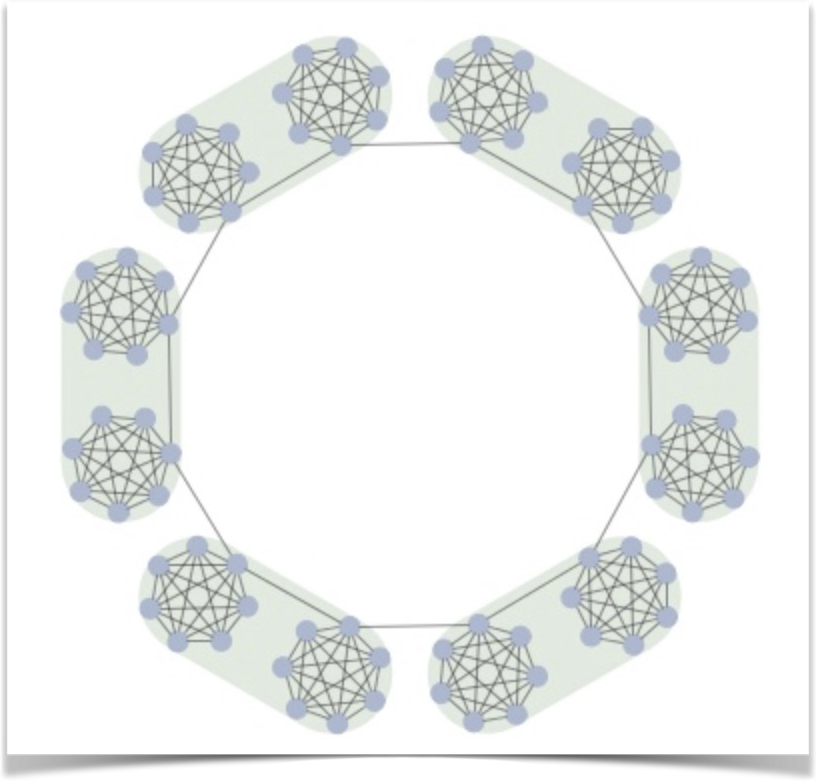
\includegraphics[width=0.7\textwidth]{ringclique.png}
\end{textbox}

\begin{textbox}{Modularity and random networks}
Another well known limitation of a Modularity maximization approach is that it finds communities with high scores in random networks: since it is not \textit{adjusted for chance}, random flucutations in a random network are mistaken for meaningful structure in the network.
\end{textbox}

\begin{textbox}{Multi-resolution Modularity}
A simple solution has been proposed to the limit of resolution, consisting in adding a resolution parameter $\lambda$ to \textit{tune} the desired resolution\cite{reichardt2006statistical}, i.e., $(L_{i}-\frac{1}{2}K_i^2)$ becomes $(L_{i}-\lambda \frac{1}{2}K_i^2)$. It raises of shrink the expected number of edges inside communities. It requires, however, to choose a proper value for $\lambda$, i.e., to choose arbitrarily a scale for communities.
\end{textbox}

\begin{textbox}{Modularity maximization: Girvan Newman}
Several of the most popular community detection algorithms have as objective to discover the partition of highest modularity. This is a difficult problem, and thus existing approaches are based on heuristics. 

The first method by Girvan and Newman \footcite{girvan2002community} first build a dendromgram by iteratively removing edges of highest betweenness. It is called a \textit{divise} approach: At the top of the dendrogram, there is a single community, then 2, 3, 4 etc., until each node is in its own community. Modularity is used as a criterium to \textit{cut} the dendrogram. 

\centering
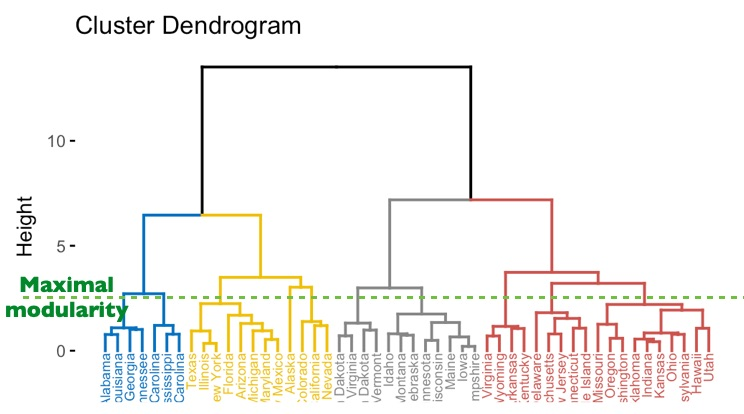
\includegraphics[width=0.7\textwidth]{dendrogram.jpg}

\end{textbox}

\begin{textbox}{Modularity maximization: Louvain method}
The Louvain method\footcite{blondel2008fast} is certainly the most used method for community detection. Its objective is to optimize the modularity using a greedy, agglomerative approach, composed of two steps: 

\textbf{Step 1}: Optimizing modularity at a hierarchical level
\begin{itemize}
    \item Each node starts in its own community
    \item Repeat until convergence:
    \begin{enumerate}
        \item \textbf{FOR} each node, compute the gain in modularity of adding it to the community of each of its neighbors
        \item choose the decision that increase the most the modularity (the best decision can be to remain in the same community
    \end{enumerate}
\end{itemize}

\textbf{Step 2}: Global algorithm
\begin{itemize}
    \item Repeat until convergence:
    \begin{enumerate}
        \item Optimize modularity for the current hierarchical level
        \item Move to a higher hierarchical level by computing an \textbf{induced network}: Each community becomes a node, the weight of the edge between nodes/communities $i$ and $j$ corresponds to the number of edges between nodes of $c_i$ and nodes of $c_j$.
    \end{enumerate}
\end{itemize}

The result of Louvain algorithm is therefore a \textbf{hierarchy} of communities. 

The main reason explaining the popularity of the Louvain method to this day is its
   \textbf{scalability}: The algorithm is very efficient in practice on real graphs, for several reasons: 1)It is a greedy approach,2) By checking only the interest of moving to neighbor's communities, it benefits from the sparsity of networks, 3)Modularity gains of a partition change can be computed locally, using its definition as a sum of independent values for each community.

\end{textbox}


\begin{textbox}{Infomap}
Infomap\cite{rosvall2008maps} is a method based on an objective function different from the Modularity. Its objective is to \textbf{Minimize the description of an average random walk} in the network, i.e. maximize the \textbf{compression} of the description of such a walk. More formally, the code length to minimize for partition $M$ is described as:
\[
H(M)=qH(\curvearrowright)+\sum_i^Cp^iH(\circlearrowright_i)
\]
with $q$ the probability for a move to be between modules,$H(\curvearrowright)$ the information required to encode a move between modules, $p^i$ the probability for a move to be inside community $i$ and $H(\circlearrowright_i)$ the information required to encode a move inside community $i$

A greedy optimization algorithm, similar in nature to the one of Louvain, is then used to minimize this description length.

Compared with Modularity, the main advantage of this approach is that it does not find communities in random networks. It is known also to suffer from a resolution limit, although not exactly similar to the one of Modularity.
\end{textbox}

\begin{textbox}{Stochastic Block Models (SBM)}
A stochastic block model is a random graph model defined by:
\begin{itemize}
\item $k$: number of blocks 
    \item $b$ a $n\times 1$ vector such as $b_i$ describes the index of the block of node $i$.
    \item $E$ a $k\times k$ \textbf{stochastic block matrix}, such as $E_{ij}$ gives the number of edges between blocks $i$ and $j$ (or equivalently, the probability to observe an edge between any pair of nodes chosen with one node in each of the two blocks).
\end{itemize}
\end{textbox}

\begin{textbox}{SBM inference}
The objective of a community/block detection algorithm based on this principle is thus to perform \textbf{SBM inference}, i.e., to find the parameters of the SBM that best explain the observed graph, usually in term of maximizing the likelihood. Said differently, we search --among a certain class of models-- the model that has the highest probability to generate the observed graph. Note that for an observed graph, for each partition in blocks $b$, there is a single block matrix $E$ that is relevant to consider, that can be found simply by counting the number of edges actually present between blocks in the graph.  

More formally, the objective is:
\[
b:=\argmax_{b} P(A|b)
\]

Note that with this formulation, it is not possible to infer the number of clusters $k$, since the trivial solution in which each node belongs to its own block, with $E=A$ has a maximal probabity (1) to generate the observed graph. The desired number of clusters is thus a necessary parameter of SBM inference.
\end{textbox}






\begin{textbox}{SBM with inference of the number of blocks}
Recently, new approaches\footcite{peixoto2019bayesian} have been proposed to be able to infer also the number of blocks. They adopt an approach from Information Theory called the Minimum Description Length (MDL), whose principle is to find the description which reduces the total cost of describing a graph, by minimizing both 1)The quantity of information needed to encode the graph, knowing that it is generated by a given model, and 2)The quantity of information needed to encode the model itself. Intuitively, a model with few blocks requires little information to be described, contrary to a model with many blocks. But a model with many block is more \textbf{constrained}, the graphs it generates are more \textit{specific}, and therefore can be described at a lesser cost, knowing the model.

More formally, we can decompose the probability of observing a graph and a model as $P (A, k, e, b) = P (A|k, e, b)P (k|e, b)P (e|b)P (b)$ with the last three probability being \textit{priors}.  Said differently, we can define the number of bits required to encode a model as $L = -log_2 P(k,b)$, the number of bits necessary to encode a graph knowing the model as $S = -log_2 P(A|k,b)$ and thus the total cost to minimize as $S+L$. The objective thus becomes:
\[
b:=\argmin_{b} - log_2 P(k,b) - log_2 P(A|k,b)
\]

\end{textbox}





\begin{textbox}{Variants of the SBM}
Group inference using SBM is a very active field of research, and many variants have been proposed, including degree-corrected, nested, Overlapping, Mixed membership SBM, etc.

An introduction to the state of the art can be found for instance in \footcite{lee2019review}.

A python library \footnote{https://graph-tool.skewed.de} exists to apply recent methods to observed graphs.
\end{textbox}



\begin{textbox}{Evaluation of Community structures}
Since there isn't a unique accepted definition of what are good communities, the evaluation of the quality of a partition or set of communities is not a trivial task. 

There are two main approaches:
\begin{itemize}
    \item \textbf{Internal evaluation} consists in using \textit{quality functions} (e.g., Modularity) to give a score for a pair partition-graph
    \item \textbf{External evaluation} consists in comparing a computer partition to a \textbf{ground truth} reference partition.
\end{itemize}
\end{textbox}

\begin{textbox}{Internal Evaluation}
Several quality functions exist to evaluation the quality of a community partition of a graph. They can therefore be understood as different \textit{definitions} of communities. While some methods try directly to optimize one of those quality functions, some other methods are based on different principles (e.g., clique-based communities, consensus reaching based on game-theory, etc.). Quality functions can therefore be used a posteriori to assess the quality of communities they found. 

The most popular are:
\begin{itemize}
    \item \textbf{Modularity}
    \item \textbf{Information compression}, as in Infomap or SBM
    \item \textbf{Surprise} \cite{aldecoa2013surprise} evaluates the departure of the observed partition from the expected distribution of nodes and links into communities given a null model, and is therefore related to modularity 
\end{itemize}, Conductance, , cut-ratio, and Surprise.

Some other quality functions are defined \textbf{for individual communities}, although they can be combined to provide a global score. The most popular are\footnote{leskovec2010empirical}:
\begin{itemize}
    \item \textbf{Conductance}, the fraction of all stubs of nodes in the community that points outside of it
    \item \textbf{ODF}, Out Degree Fraction, the average for every node of its fraction of neighbors inside the community
    \item \textbf{Internal Transitivity}, the clustering coefficient inside the community
    \item \textbf{Scaled density}, the ratio of the node density to the total graph density
\end{itemize}


\end{textbox}

\begin{textbox}{External Evaluation}
Partitions obtained by a given method can be compared with a ground truth. This approach is used on real networks, with a ground truth coming from metadata (e.g., classes in a network of social interactions between students), and on synthetic networks, with communities known by construction.

Although this is still discussed in the literature, it is mostly accepted that the evaluation on real networks using this approach is problematic\footcite{peel2017ground}, because there is no guarantee that the labels used as ground truth are indeed related to the \textbf{topological structure} of the network, which is what communities are about.

Most popular methods for partitions comparisons are:
\begin{itemize}
\item \textbf{NMI}, Normalized Mutual Information, and its adjusted for chance variant, \textbf{AMI}.
\item \textbf{ARI}, Adjusted Rand Index
\end{itemize}
But more generally, any method for cluster comparison can be used\footcite{dao2020community}
\end{textbox}


\begin{textbox}{Overlapping communities}
For many types of networks, the real organization of networks is thought to be overlapping, i.e., each node can belong to several communities. Think of your personal social networks: some of your family members might also be part of a group of friends, or some of your friends from high school might also be part of your friends from university, which are otherwise distinct groups. 

Detecting overlapping clusters is considered harder than non-overlapping ones, for two reasons: the search space (number of possible solutions) is much larger (and even infinite), and defining what good communities are is even harder, since there isn't the natural limit for each edge to be either internal or external.

A large number of methods have nevertheless been proposed\footcite{xie2013overlapping}. Extensions of non-overlapping quality functions have been proposed, such as the overlapping Modularity \footcite{nicosia2009extending}, or overlapping NMI \footcite{mcdaid2011normalized}.
\end{textbox}

\begin{textbox}{Other meso-scale structures}
Beyond the community structures we have alredy defined, other types of network structural organization have been proposed and studied. Some of the most widely known are:
\begin{itemize}
    \item \textbf{Link communities}, in which communities are defined as \textit{sets of links}. Searching for (non-overlapping) partitions of edges yield a structure in which nodes naturally belong to several groups, i.e., a community can correspond to \textit{familial} edges, another to \textit{professional} edges, etc. (\cite{ahn2010link})
    \item \textbf{Fuzzy communities}, in which nodes belong to (often several) communities with a certain probability or strength (\cite{liu2010fuzzy})
    \item \textbf{Core-Periphery structure}, already defined when we introduce the notion of \textit{k-cores}
    \item \textbf{Nestedness}, corresponding to a network with a hierarchical organization such as elements with few connections tends to be connected to a subset of the neighbors of a \textit{parent} node. (\cite{pawar2014plant})
    \item \textbf{Spatial organization}, in which the probability of observing an edge between nodes depends on their distance. (\cite{barthelemy2011spatial})
\end{itemize}
\end{textbox}